\documentclass[11pt]{article}\usepackage[]{graphicx}\usepackage[]{color}
% maxwidth is the original width if it is less than linewidth
% otherwise use linewidth (to make sure the graphics do not exceed the margin)
\makeatletter
\def\maxwidth{ %
  \ifdim\Gin@nat@width>\linewidth
    \linewidth
  \else
    \Gin@nat@width
  \fi
}
\makeatother

\definecolor{fgcolor}{rgb}{0.345, 0.345, 0.345}
\newcommand{\hlnum}[1]{\textcolor[rgb]{0.686,0.059,0.569}{#1}}%
\newcommand{\hlstr}[1]{\textcolor[rgb]{0.192,0.494,0.8}{#1}}%
\newcommand{\hlcom}[1]{\textcolor[rgb]{0.678,0.584,0.686}{\textit{#1}}}%
\newcommand{\hlopt}[1]{\textcolor[rgb]{0,0,0}{#1}}%
\newcommand{\hlstd}[1]{\textcolor[rgb]{0.345,0.345,0.345}{#1}}%
\newcommand{\hlkwa}[1]{\textcolor[rgb]{0.161,0.373,0.58}{\textbf{#1}}}%
\newcommand{\hlkwb}[1]{\textcolor[rgb]{0.69,0.353,0.396}{#1}}%
\newcommand{\hlkwc}[1]{\textcolor[rgb]{0.333,0.667,0.333}{#1}}%
\newcommand{\hlkwd}[1]{\textcolor[rgb]{0.737,0.353,0.396}{\textbf{#1}}}%
\let\hlipl\hlkwb

\usepackage{framed}
\makeatletter
\newenvironment{kframe}{%
 \def\at@end@of@kframe{}%
 \ifinner\ifhmode%
  \def\at@end@of@kframe{\end{minipage}}%
  \begin{minipage}{\columnwidth}%
 \fi\fi%
 \def\FrameCommand##1{\hskip\@totalleftmargin \hskip-\fboxsep
 \colorbox{shadecolor}{##1}\hskip-\fboxsep
     % There is no \\@totalrightmargin, so:
     \hskip-\linewidth \hskip-\@totalleftmargin \hskip\columnwidth}%
 \MakeFramed {\advance\hsize-\width
   \@totalleftmargin\z@ \linewidth\hsize
   \@setminipage}}%
 {\par\unskip\endMakeFramed%
 \at@end@of@kframe}
\makeatother

\definecolor{shadecolor}{rgb}{.97, .97, .97}
\definecolor{messagecolor}{rgb}{0, 0, 0}
\definecolor{warningcolor}{rgb}{1, 0, 1}
\definecolor{errorcolor}{rgb}{1, 0, 0}
\newenvironment{knitrout}{}{} % an empty environment to be redefined in TeX

\usepackage{alltt}
%\usepackage[showframe]{geometry}
\usepackage{caption}
\usepackage{lscape,verbatim,mathrsfs}
\usepackage{graphics,amsmath,pstricks}
\usepackage{amssymb,enumerate}
\usepackage{amsbsy,amsmath,amsthm,amsfonts, amssymb}
\usepackage{graphicx, rotate, array}
\usepackage{geometry,multirow}
\usepackage{color,soul}
\usepackage{float}
\usepackage{datetime}
%\usepackage{hyperref}
\usepackage[authoryear,round]{natbib}
%\renewcommand{\baselinestretch}{1.9}
\usepackage{tcolorbox}
\renewcommand{\familydefault}{cmss}
\textwidth=6.65in \textheight=9.7in
\parskip=.025in
\parindent=0in
\oddsidemargin=-0.1in \evensidemargin=-.1in \headheight=-.6in
\footskip=0.5in \DeclareMathOperator*{\argmax}{argmax}
\DeclareMathOperator*{\argmin}{argmin}
\IfFileExists{upquote.sty}{\usepackage{upquote}}{}
\begin{document}
%\SweaveOpts{concordance=TRUE}
\part*{Primary Analysis Objective 4 for Viral Suppression}
\today
\currenttime

Definition: outcome $Y$ is indicator that person was virally suppressed at year 2 (i.e., $Y = 1$ if person suppressed, $Y=0$ if non-suppressed). People with missing $Y$ were excluded. 




%\section{Start = initial randomization, End = 2 years after enrollment}



\section{15 Sequential Interventions}

\subsection{With Simultaneous CIs}
\begin{knitrout}
\definecolor{shadecolor}{rgb}{0.969, 0.969, 0.969}\color{fgcolor}\begin{kframe}
\begin{verbatim}
        Type Int Estimates   lowerCI   upperCI
1  Min. adj.   1 0.7515450 0.6871121 0.8159778
2  Min. adj.   2 0.7759425 0.6974158 0.8544693
3  Min. adj.   3 0.8029829 0.7395310 0.8664347
4  Min. adj.   4 0.8072552 0.7446310 0.8698795
5  Min. adj.   5 0.7725896 0.7011875 0.8439917
6  Min. adj.   6 0.8110646 0.7428767 0.8792525
7  Min. adj.   7 0.7874045 0.7244287 0.8503802
8  Min. adj.   8 0.8262360 0.7561243 0.8963477
9  Min. adj.   9 0.8312647 0.7713522 0.8911772
10 Min. adj.  10 0.7652299 0.6875713 0.8428886
11 Min. adj.  11 0.7288946 0.6599580 0.7978313
12 Min. adj.  12 0.7618770 0.6912343 0.8325198
13 Min. adj.  13 0.7369763 0.6636932 0.8102595
14 Min. adj.  14 0.8155234 0.7464896 0.8845572
15 Min. adj.  15 0.7571764 0.6910365 0.8233164
16 Full adj.   1 0.7467291 0.6837448 0.8097134
17 Full adj.   2 0.7830515 0.7087381 0.8573650
18 Full adj.   3 0.8048698 0.7436033 0.8661362
19 Full adj.   4 0.7977028 0.7348310 0.8605745
20 Full adj.   5 0.7780551 0.7091719 0.8469383
21 Full adj.   6 0.8138591 0.7506124 0.8771059
22 Full adj.   7 0.7925117 0.7323927 0.8526307
23 Full adj.   8 0.8275302 0.7617456 0.8933149
24 Full adj.   9 0.8300798 0.7717358 0.8884238
25 Full adj.  10 0.7646551 0.6923299 0.8369803
26 Full adj.  11 0.7286561 0.6621923 0.7951199
27 Full adj.  12 0.7581491 0.6914951 0.8248031
28 Full adj.  13 0.7350985 0.6661322 0.8040648
29 Full adj.  14 0.8099981 0.7472797 0.8727165
30 Full adj.  15 0.7531579 0.6892224 0.8170934
\end{verbatim}
\end{kframe}
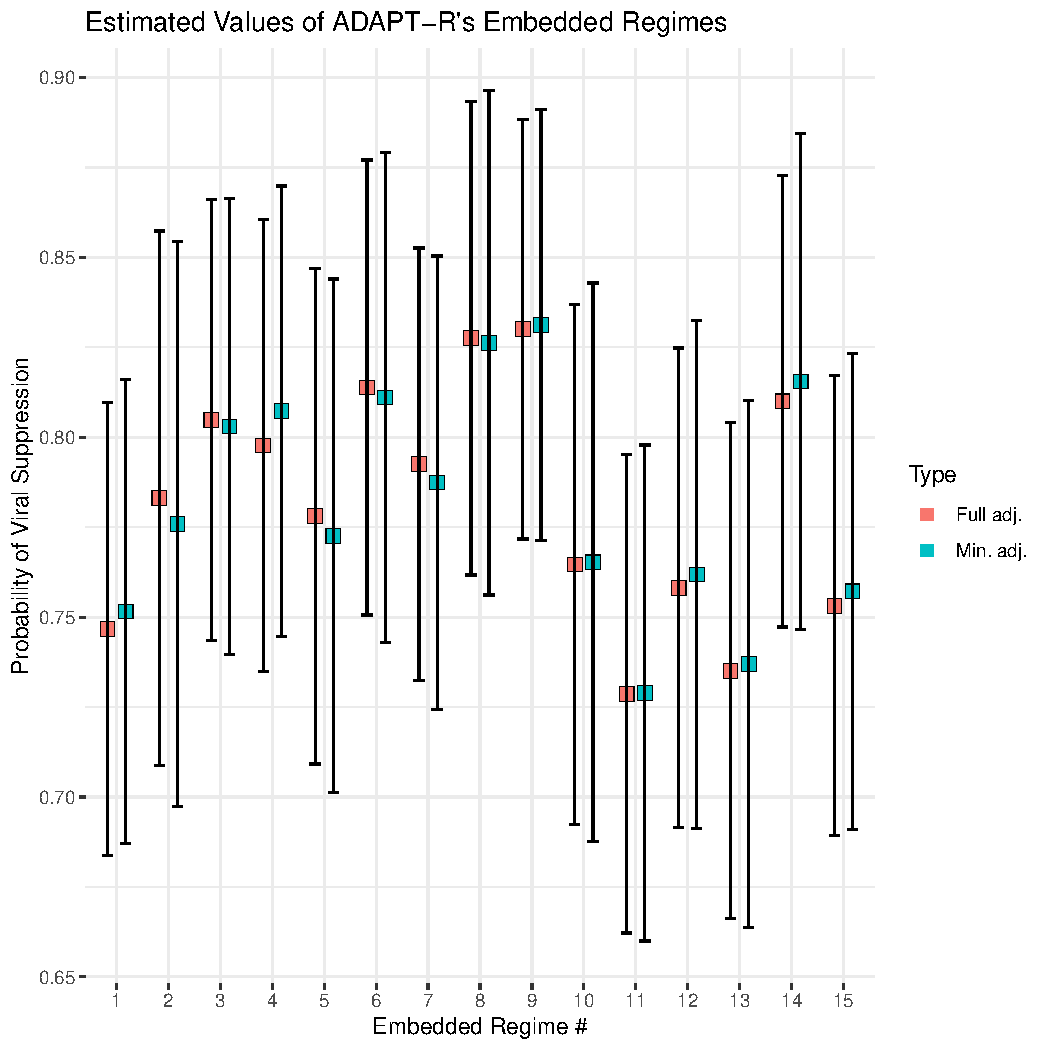
\includegraphics[width=\maxwidth]{figure/unnamed-chunk-2-1} 
\begin{kframe}\begin{verbatim}
pdf 
  2 
\end{verbatim}
\end{kframe}
\end{knitrout}

Width of Min. Adj. CIs are this times larger than Full. Adj. CIs
\begin{knitrout}
\definecolor{shadecolor}{rgb}{0.969, 0.969, 0.969}\color{fgcolor}\begin{kframe}
\begin{verbatim}
[1] 0.9960641 1.1006944
\end{verbatim}
\end{kframe}
\end{knitrout}

\begin{knitrout}
\definecolor{shadecolor}{rgb}{0.969, 0.969, 0.969}\color{fgcolor}\begin{kframe}
\begin{verbatim}
voucher_navigator_continue 
                 0.8300798 
CI_simult           
0.7717358 0.8884238 
voucher_outreach_stop 
            0.7286561 
CI_simult           
0.6621923 0.7951199 
\end{verbatim}
\end{kframe}
\end{knitrout}

Contrasts
\begin{knitrout}
\definecolor{shadecolor}{rgb}{0.969, 0.969, 0.969}\color{fgcolor}\begin{kframe}
\begin{verbatim}
diff.sms_sms.voucher_continue                           CI1 
                   0.03132595                   -0.03198123 
                          CI2 
                   0.09463313 
diff.voucher_sms.voucher_continue                               CI1 
                      0.067129979                       0.006620345 
                              CI2 
                      0.127639612 
diff.sms_navigator_continue                         CI1 
                 0.08080108                  0.01898748 
                        CI2 
                 0.14261469 
diff.voucher_navigator_continue                             CI1 
                     0.08335066                      0.02508373 
                            CI2 
                     0.14161759 
diff.voucher_outreach_stop                        CI1 
               -0.01807308                -0.08020119 
                       CI2 
                0.04405504 
\end{verbatim}
\end{kframe}
\end{knitrout}







\end{document}
